\chapter{Supervised Learning Model}
\section{Mô hình:}
\begin{figure}[H]
    \centering
    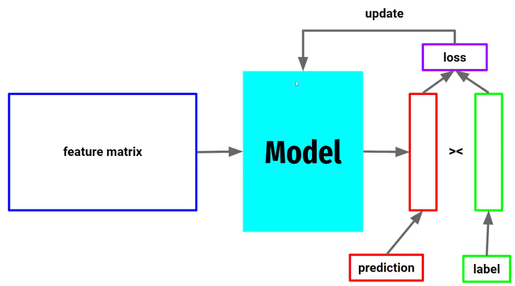
\includegraphics[width=0.8\linewidth]{01.png}
    \caption{Mô hình Supervised Learning}
    \label{fig: mdl_spl}
\end{figure}
\begin{itemize}
    \item \textbf{Giải thích mô hình:}
    \begin{itemize}
        \item Future matrix: Ma trận thuộc tính.
        \item Prediction: Kết quả từ mô hình.
        \item Label: Kết quả mong muốn.
        \item Loss: Hàm mất mát cho biết mức độ chênh lệch giữa Prediction và Label
        \begin {itemize}
            \item Loss thấp: Mô hình có độ chính xác cao.
            \item Loss cao: Ngược lại.
        \end {itemize}
        \item Loss luôn cập nhật mục đích để phản ánh lại prediction
    \end{itemize}
\end{itemize}

\section{Loss Function:}
\begin{figure}[H]
    \centering
    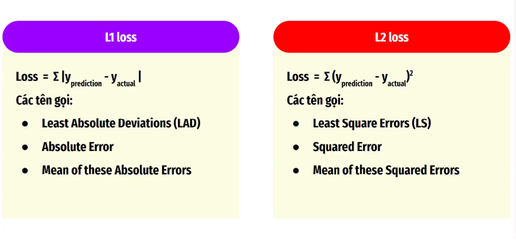
\includegraphics[width=0.8\linewidth]{02.png}
    \caption{Hàm mất mát (Loss Function)}
    \label{fig:loss_func}
\end{figure}
\subsection {Câu hỏi:}
\begin{itemize}
    \item Tại sao lại có hai hàm Loss?
    \item Sử dụng hàm như thế nào cho đúng?
\end{itemize}
\subsection {L1: Mong muốn mô hình phải thật chính xác, tối đa hoá sự chính xác:}
\begin{itemize}
    \item Thu được các sai số rất nhỏ với $y-hat$ chính xác cao.
    \item Tối đa hoá giá trị prediction với độ chính xác cao.
    \item Chấp nhận một vài outlier.
    \item Hạn chế tác động của Outlier (Không bị chi phối).
    \item Dùng cho trường hợp data bị nhiễu nhiều outlier.
\end{itemize}

\subsection {L2: Mong muốn mô hình với sai số tối thiểu, tối thiểu hoá sai số}
\begin{itemize}
    \item Sẽ nghiêm trọng với sai số lớn vì sai số sẽ bình phương lên.
    \item Mô hình sẽ tập trung vào những điểm outlier, kéo lệch kết quả dự đoán.
    \item Dùng cho bài toán có dữ liệu sạch.
\end{itemize}

\section{Phân chia dữ liệu trong ML pipeline}
\begin{figure}[H]
    \centering
    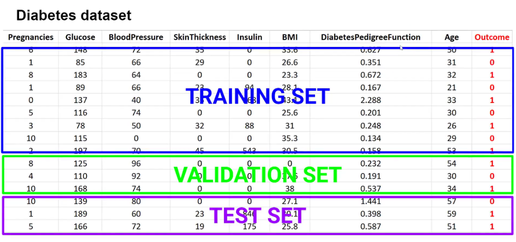
\includegraphics[width=0.8\linewidth]{03.png}
    \caption{Phân chia dữ liệu}
    \label{fig:dataset_devide}
\end{figure}

\begin{itemize}
    \item Trainning set: Dùng để huấn luyện mô hình, có khả năng làm mô hình tốt hơn nếu data càng lớn.
    \item Validation set: Kiểm tra quá trình huấn luyện, kết quả thu được dùng để cải thiện model.
    \item Test set: Kiểm tra performance của model.
\end{itemize}

\section{Classification metrics}
\begin{figure}[H]
    \centering
    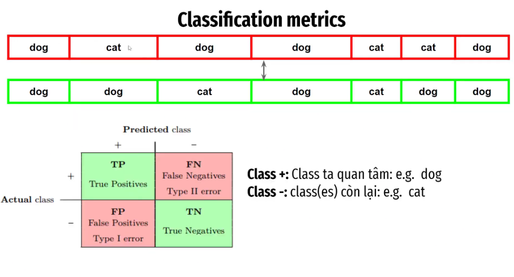
\includegraphics[width=0.8\linewidth]{04.png}
    \caption{Chia dữ liệu dựa trên mối quan tâm}
    \label{fig: class_devide}
\end{figure}
\begin{itemize}
    \item Metrics của classification: Dùng để đánh giá mô hình.
    \item Các metric thường sử dụng.
\end{itemize}
\begin{figure}[H]
    \centering
    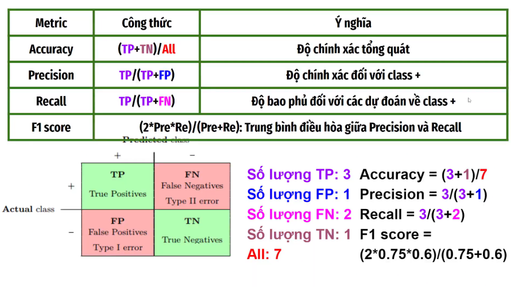
\includegraphics[width=0.8\linewidth]{05.png}
    \caption{Classification metrics}
    \label{fig:cl_metrics}
\end{figure}
\begin{itemize}
    \item Giải thích:
    \begin{itemize}
        \item Accuracy: Độ chính xác tổng quát.
        \item Precision: Đối với nhóm dương tính thì có bao nhiêu kết quả thực sự chính xác (Nhóm cụ thể).
        \item Recall: Có bao nhiêu dự đoán chính xác trên số lượng chính xác trong thực tế (Ví dụ : Trong số người thực sự dương tính  thì có bao nhiêu người được dự đoán chính xác dương tính).
        \item F1 score: Trung bình điều hòa Precision và Recall, dùng để đánh giá trong trường hợp dữ liệu mất cân bằng.
    \end{itemize}
\end{itemize}

\begin{figure}[H]
    \centering
    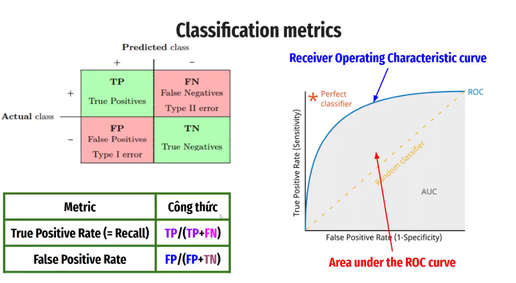
\includegraphics[width=0.8\linewidth]{06.png}
    \caption{Classification metrics}
    \label{fig:cl_metrics2}
\end{figure}
\begin{itemize}
    \item Giải thích:
    \begin{itemize}
    \item ROC: Tìm điểm tối ưu.
    \item AUC: Tìm đường tối ưu.
    \item False Positive Rate :Có bao nhiêu báo động giả(dự đoán sai) trên tổng số người âm tính thực tế. (Ví dụ : Trong tổng số người thực sự âm tính có bao nhiêu người đã bị dự đoán là dương tính).
    \end{itemize}
\end{itemize}

\begin{figure}[H]
    \centering
    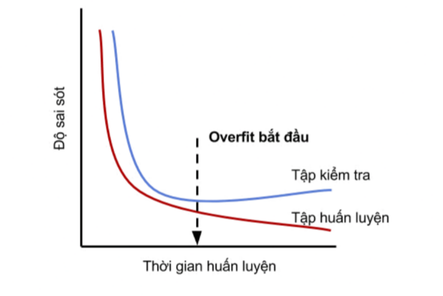
\includegraphics[width=0.8\linewidth]{07.png}
    \caption{Trainning line}
    \label{fig:trainning_line}
\end{figure}
\begin{itemize}
    \item Hiện tượng \textbf{Overfitting}: Train tốt nhưng Test kém.
    \item Ép máy tính mô phỏng lại chính xác tất cả những gì được học đồng thời cũng muốn nó có thể làm đúng được những gì chưa từng nhìn thấy dựa trên những gì đã được học, sáng tạo ra những điểm chưa tồn tại.
\end{itemize}




